\documentclass[11pt,a4paper]{article}
\usepackage[utf8]{inputenc}
\usepackage[margin=2.5cm]{geometry}
\usepackage{amsmath,amssymb}
\usepackage{booktabs}
\usepackage{xcolor}
\usepackage{graphicx}
\usepackage{caption}
\usepackage{enumitem}
\usepackage{natbib}
\usepackage[colorlinks=true,linkcolor=blue!50!black,citecolor=blue!50!black,urlcolor=blue!50!black,pdftitle={Relational Gravitational Dynamics: a one-parameter radial term, g-dagger(z) tests and the cosmological limits of the kernel},pdfauthor={Karlos Marden Maia}]{hyperref}
\setlength{\parskip}{0.45em}
\setlength{\parindent}{0pt}
\captionsetup{font=small,labelfont=bf}
\newcommand{\gdag}{g^{\dagger}}
\newcommand{\Keff}{K_{\rm eff}}
\newcommand{\Msun}{M_\odot}
\newcommand{\fbar}{f_{\rm bar}}
\newcommand{\fgas}{f_{\rm gas}}

\begin{document}

\begin{center}
{\LARGE\bfseries Relational Gravitational Dynamics:\\[0.3em] a one-parameter radial term, tests of $\gdag(z)$,\\[0.3em] and the cosmological limits of the kernel}\\[1.2em]
{\large Unifying disk galaxies, galaxy groups and galaxy clusters\\ under a single effective law --- second paper}\\[1.5em]
{\large Karlos Marden Maia}\\
Independent Researcher $\cdot$ Marietta, Georgia, USA\\[0.8em]
October 22, 2026\\[0.4em]
{\small Version 5 (supersedes v4 of April 28, 2026)}
\end{center}
\vspace{0.8em}

\begin{abstract}
\noindent
The effective gravitational kernel of the previous version (v4) describes the ratio of observed to baryonic acceleration in bound systems with $\Keff = 1+\lambda e^{-x}/(1-e^{-x})^{n}$, $x=g_{\rm bar}/\gdag(z)$, $\gdag=cH(z)/2\pi$ and $n(\xi)=\tfrac12+A\xi$. Its radial extension, an exponent modulation $w^{-\alpha(\xi)}$ with two extra parameters calibrated on a subset of the same data, was left as a semi-predictive result. Here the radial dependence is replaced by a scale shift $s=[\Delta(r)/\Delta_{500}]^{\,p\,\Theta(\xi-\xi_c)}$, where $\Delta/\Delta_{500}=\bar\rho(<r)/500\rho_c$, with one parameter ($p\simeq0.45$--$0.5$) and a step in the compactness $\xi$ that switches the term on in groups and clusters and off in galaxies. On the 39 X-COP radial points used in v4 the rms falls from 0.037 to 0.016--0.021 dex; unlike the v4 law, the new term remains finite inside $r_{500}$: with Vikhlinin et al.\ (2006) it predicts $\fbar(r_{2500})/\fbar(r_{500})=1.00$ against $0.90$ observed (v4 law: 1.95; no radial term: 3.37), and with measured gas fractions out to $r_{200}$ (Ettori et al.\ 2019) it predicts $0.97$ against $1.03$. The evolution $\gdag\propto H(z)$ is preferred by measured gas fractions in the Allen et al.\ (2008) and Mantz et al.\ (2014) samples (a frozen $\gdag$ is rejected by $\Delta\chi^2=57$ and 48), whereas median KMOS$^{\rm 3D}$ galaxies at $z\simeq0.9$--2.3 favour a weaker evolution ($\gdag\propto E^{0.5\text{--}0.75}$), a difference within the $\sim10\%$ systematics. We document four unresolved tensions: the baryon fraction at $r_{2500}$ rises with mass more steeply than observed; the absolute normalisation differs by $\sim20\%$ between the Chandra and XMM samples; a mass-dependent exponent $p(\xi)$ is disfavoured; and the high-redshift galaxy trend. Applied to linear cosmological perturbations the kernel boosts gravity by factors $10^2$--$10^3$ and destroys linearity; a density-based damper restores $\Lambda$CDM growth only by postulating the plateau $K_c=\Omega_m/\Omega_b$. The program remains an explicitly phenomenological map of bound systems, competitive with $\Lambda$CDM in clusters, parsimonious but poorer in fit in galaxies, and silent on the CMB.
\end{abstract}

\noindent\textbf{Keywords:} dark matter alternatives $\cdot$ modified gravity $\cdot$ galaxy clusters $\cdot$ radial acceleration relation $\cdot$ baryon fraction $\cdot$ Tully--Fisher relation $\cdot$ cosmological evolution of $\gdag$

\tableofcontents
\newpage

%--------------------------------------------------------------------
\section{Introduction}
The kernel proposed in the first paper of this program (v4, hereafter Paper~I) maps the baryonic acceleration $g_{\rm bar}$ of a bound system to its observed acceleration, $g_{\rm obs}=\Keff\,g_{\rm bar}$, using a transition scale $\gdag(z)=cH(z)/2\pi$ and an exponent $n$ that depends on the equilibrium geometry through the compactness $\xi=g_{500}/\gdag(z)$. Paper~I tested it on SPARC disk galaxies, 23 groups, 13 X-COP clusters and 23 CLASH clusters and listed its own limitations. Four of them are the subject of this work.

\begin{enumerate}[leftmargin=2em,itemsep=0.1em]
\item \emph{The radial law was semi-predictive.} The factor $w^{-\alpha(\xi)}$, with $\alpha(\xi)=0.355(1-e^{-\xi/0.052})$, used two parameters derived earlier from a subset of eight X-COP clusters, and the 39-point test of Paper~I partially overlaps that calibration. Paper~I lists validation on resolved profiles, with a falsification criterion of 0.10 dex, as an open item.
\item \emph{The evidence for $\gdag\propto H(z)$ rested on CLASH gas fractions estimated from a scaling relation.} Paper~I itself discusses whether part of the residual correlation is algebraic.
\item \emph{Groups were 23 and no variable switched the radial term between galaxies and clusters.}
\item \emph{No test at high redshift and no treatment of cosmological scales} were given; the extension was declared outside the scope.
\end{enumerate}

We (i) replace the radial law by a one-parameter scale shift and compare it with the v4 law on the same and on independent data (Sect.~\ref{sec:radial}); (ii) test $\gdag(z)$ with measured gas fractions and with $z\simeq1$--2 galaxies (Sect.~\ref{sec:gz}); (iii) introduce a step in $\xi$ connecting galaxies to groups and clusters and derive its redshift dependence (Sect.~\ref{sec:switch}); (iv) compare with $\Lambda$CDM (Sect.~\ref{sec:lcdm}); (v) document the tensions (Sect.~\ref{sec:tensions}); and (vi) examine what happens when the kernel is applied to cosmological perturbations and how a density-based damper behaves (Sect.~\ref{sec:cosmo}). Section~\ref{sec:disc} states what the program does and does not claim, and lists falsifiable tests.

%--------------------------------------------------------------------
\section{The kernel and its radial extension}
\label{sec:model}
\subsection{Definition}
For a bound, spherically or axially symmetric system in equilibrium,
\begin{equation}
\Keff = 1+\frac{\lambda\,e^{-x/s}}{\left(1-e^{-x/s}\right)^{n}},\qquad x=\frac{g_{\rm bar}}{\gdag(z)},\qquad \gdag(z)=\frac{cH(z)}{2\pi},
\label{eq:K}
\end{equation}
with $\lambda=0.999$, $H_0=70\ {\rm km\,s^{-1}\,Mpc^{-1}}$, $\Omega_m=0.3$, and the exponent law of Paper~I,
\begin{equation}
n(\xi)=\tfrac12+A\,\xi,\qquad A=0.4068,\qquad \xi=\frac{g_{500}}{\gdag(z)}=\frac{2\pi\,G M_{500}}{c\,H(z)\,R_{500}^2}.
\label{eq:n}
\end{equation}
For $s=1$ and $\xi\to0$ this is the disk-galaxy kernel ($n=1/2$) with the baryonic Tully--Fisher relation $v_f^4=\lambda^2\gdag G M_b$ as a structural consequence. The compactness $\xi$ scales as $(MH)^{1/3}$.

\subsection{Radial term}
Paper~I modulated the exponent, $n\to n(\xi)\,w^{-\alpha(\xi)}$ with $w=r/R_{500}$. Here the exponent is kept at its $w=1$ value and the radial dependence enters through the scale $s$,
\begin{equation}
s=\left[\frac{\Delta(r)}{\Delta_{500}}\right]^{p\,\Theta(\xi-\xi_c)},\qquad \frac{\Delta(r)}{\Delta_{500}}=\frac{\bar\rho(<r)}{500\,\rho_c(z)}=\frac{M(<r)}{M_{500}}\left(\frac{R_{500}}{r}\right)^{3}.
\label{eq:s}
\end{equation}
By definition $\Delta/\Delta_{500}=1$ at $r_{500}$, $5$ at $r_{2500}$ and $0.4$ at $r_{200}$, so $p$ is the only radial parameter and the $w=1$ calibration of Paper~I is untouched. $\Theta$ is a step in $\xi$, implemented as $\Theta=[1+(\xi_c/\xi)^m]^{-1}$ with $m\ge32$, and $\xi_c$ is bracketed by the data (Sect.~\ref{sec:switch}). Systems with $\xi<\xi_c$ have $s=1$.

\subsection{Self-consistent baryon fraction}
In a system with total enclosed mass $M(<r)$ and baryonic fraction $f=M_{\rm bar}/M$, $g_{\rm obs}=GM/r^2$ and $x=f\,g_{\rm obs}/\gdag$; the identity $K=g_{\rm obs}/g_{\rm bar}=1/f$ gives the equation $f\,K(f\,g_{\rm obs}/\gdag)=1$, solved for $f$. The prediction is a baryon fraction, which is compared with the observed gas plus stellar fraction. Because the observable depends on the measured total mass, hydrostatic masses are interpreted as the effective dynamical mass $g_{\rm obs}r^2/G$; they are unbiased with respect to the gravity law if the gas is in equilibrium in the potential of Eq.~(\ref{eq:K}) (Sect.~\ref{sec:tensions}).

%--------------------------------------------------------------------
\section{Data and method}
\label{sec:data}
Table~\ref{tab:samples} lists the samples. Tables for Allen, Mantz, Vikhlinin, Lovisari, Sun, Ettori and Umetsu were transcribed from the published papers (Appendix~\ref{app:repro}) and cross-checked where redundancy allows (e.g. Mantz $M_{2500}$ against the value implied by $r_{2500}$ and the critical density, median ratio 0.999; Vikhlinin $M_{500}$ against $500\rho_c(4\pi/3)r_{500}^3$, 0.96--1.02).

\begin{table}[h]
\centering\small
\begin{tabular}{p{4.1cm}p{3.0cm}p{4.9cm}p{2.2cm}}
\toprule
Sample & N & Observable & Use \\
\midrule
SPARC (Lelli et al.\ 2016), Table 2 & 175 gal.\ (2803 pts after cuts) & rotation curves & galaxies, $s=1$ \\
Lovisari+15, Sun+09 & 43 groups & $M$, $M_{\rm gas}$ at $r_{500},r_{2500}$ & transition regime \\
X-COP (Ettori+19, Eckert+19, Ghirardini+19) & 13 / 12 clusters & $M(<r)$ at 0.5, 1, 1.5 Mpc / $\fgas(r_{500},r_{200})$ & radial term \\
Vikhlinin+06 & 12 (10 with both radii) & $M_{2500}$, cumulative $\fgas$ at $r_{2500}$, $r_{500}$ & radial term at $r_{2500}$ \\
Allen+08 & 42 & cumulative $\fgas(r_{2500})$, $z\le1.1$ & $\gdag(z)$ \\
Mantz+14 & 40 & shell $\fgas$ at $0.8$--$1.2\,r_{2500}$, $z=0.08$--1.06 & $\gdag(z)$ \\
CLASH (Umetsu+16) & 12 overlapping & lensing $M_{2500}$, $M_{500}$ & HSE vs.\ lensing \\
KMOS$^{\rm 3D}$ (\"Ubler+17) & 135 gal.\ (3 bins) & $M_{\rm bar}$, $R_e$, $v_{\rm circ,max}$ at $z\simeq0.9,1.5,2.3$ & high-$z$ galaxies \\
\bottomrule
\end{tabular}
\caption{Samples. For SPARC, points with $V>0$, $R>0$ and $\sigma_V/V<0.1$ are used, with $\Upsilon_{\rm disk}=0.5$ and $\Upsilon_{\rm bul}=0.7$ for all models; the comparison with halos uses the 141 galaxies with $\ge5$ points (2736 points).}
\label{tab:samples}
\end{table}

\paragraph{Statistics.} Residuals are in $\log_{10}$ (dex) unless stated as $\ln$; model comparison uses $-2\ln L=\sum N\ln({\rm rms}^2)$ with AIC $=\sum N\ln({\rm rms}^2)+2k$, counting only the parameters added to the fixed $\lambda$, $A$, $\gdag$. When the observable measures only the redshift or radial \emph{shape} (Mantz shells, Allen cumulative fractions) the normalisation is a free scalar. Cluster stellar masses follow Kravtsov et al.\ (2018) (the relation of Gonzalez et al.\ 2013 was used only as an alternative in cross-checks), $\log M_{*,\rm tot}=12.71+0.59(\log M_{500}-14.5)$ (0.11 dex scatter, $M_{500}=4.6\times10^{13}$--$1.6\times10^{15}\,\Msun$), with a fraction $\varphi$ of it inside $r_{2500}$ ($\varphi=0.7$, 1.0 inside $r_{500}$). A hard-coded stellar fraction of 9\% of the gas is used where noted. The radial parameter $p$ and $\varphi$ are the only quantities adjusted outside the calibration of Paper~I; $\varphi$ has not been measured and is varied (0.5--0.7).

%--------------------------------------------------------------------
\section{The radial term: comparison with the v4 law}
\label{sec:radial}
\subsection{Same data as Paper I}
We reproduce the v4 test on the 39 X-COP points (13 clusters at $r=0.5,1.0,1.5$ Mpc, $w=0.35$--1.66, $f_{\rm bar}=1.09\,\fgas(M_{500})$ from the Sun et al.\ scaling relation as in Paper~I). The law $n(\xi)w^{-\alpha(\xi)}$ gives 0.037 dex (Paper~I: 0.040; the small difference may come from details of the input masses and baryon fraction that we could not reproduce exactly), fixing $n$ at $w=1$ gives 0.126, Newton alone 0.878, MOND 0.257 (Table~\ref{tab:xcop}).

\begin{table}[h]
\centering\small
\begin{tabular}{lcccccc}
\toprule
Model & extra par. & rms [dex] & 0.5 Mpc & 1.0 Mpc & 1.5 Mpc & AIC \\
\midrule
$n(\xi)$ fixed at $w=1$ & 0 & 0.126 & 0.197 & 0.062 & 0.071 & $-162$ \\
v4: $n(\xi)\,w^{-\alpha(\xi)}$ & 2 & 0.037 & 0.062 & 0.013 & 0.011 & $-253$ \\
This work, $p=0.5$ fixed & 0 & 0.021 & 0.035 & 0.006 & 0.008 & $-301$ \\
This work, $p=0.45$ fitted & 1 & 0.016 & 0.024 & 0.007 & 0.012 & $-321$ \\
NFW + Duffy $c(M)$, $M_{200}$ free & 13 & 0.039 & --- & --- & --- & $-227$ \\
\bottomrule
\end{tabular}
\caption{X-COP, 39 points. $\Delta/\Delta_{500}$ takes median values 5.2, 1.5 and 0.67 at the three radii. A leave-one-cluster-out fit gives $p=0.45$--0.46 for every omitted cluster and a predictive rms of 0.017 dex. The v4 exponent modulation and the new scale shift are both calibrated on this sample, so this comparison is not independent.}
\label{tab:xcop}
\end{table}

\begin{figure}[h]
\centering
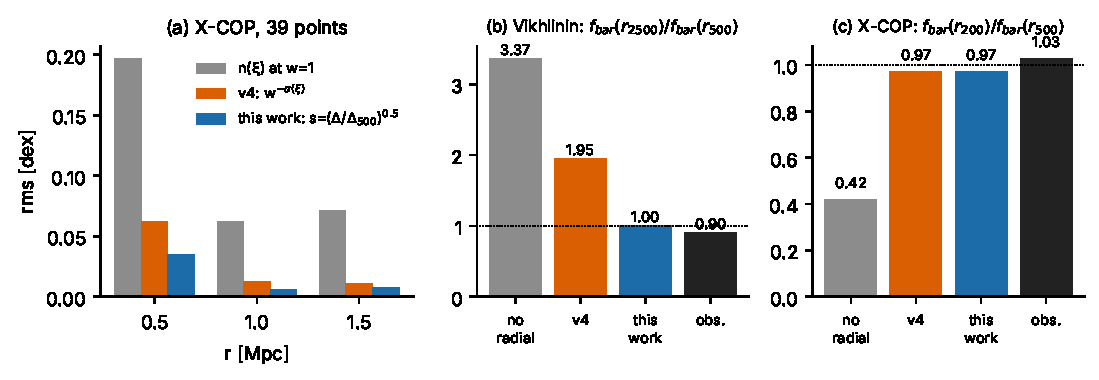
\includegraphics[width=\textwidth]{fig1_radial.pdf}
\caption{(a) rms residual by physical radius in the X-COP sample. (b) Predicted and observed $\fbar(r_{2500})/\fbar(r_{500})$ in ten Vikhlinin et al.\ clusters. (c) Same ratio at $r_{200}/r_{500}$ in nine X-COP clusters with measured $\fgas$ (Ettori et al.\ 2019). ``no radial'' denotes $n(\xi)$ at $w=1$ with $s=1$.}
\label{fig:radial}
\end{figure}

\subsection{Independent data}
\paragraph{Vikhlinin et al.\ (2006), $r_{2500}$.} For the ten clusters with cumulative $\fgas$ at both radii ($\xi=0.23$--0.59, $M_{500}=7.4\times10^{13}$--$1.1\times10^{15}\,\Msun$, $w=r_{2500}/r_{500}=0.39$--0.48) the control at $r_{500}$, where the radial term plays no role, gives obs/pred $=0.95$ (rms 0.13 in $\ln$). At $r_{2500}$ without a radial term obs/pred is 0.26 (rms$_{\ln}$ 1.35, predicted $\fbar(r_{2500})/\fbar(r_{500})=3.37$); with the v4 law 0.45 (rms$_{\ln}$ 0.90, ratio 1.95, and one of the ten clusters has no solution because $n>1$ inside $w\simeq0.45$); with the scale shift 0.84 (rms$_{\ln}$ 0.23, ratio 1.00). The observed ratio is 0.90. The v4 law, which scales the exponent as $w^{-\alpha}$, drives $n$ beyond 1 at $w<1$ for the highest $\xi$, where the kernel no longer has a finite baryon fraction; the scale shift cannot do this because it multiplies $x$ rather than the exponent. At the criterion proposed in Paper~I (0.10 dex), the v4 law with its published $\alpha(\xi)$ fails on this sample (we did not re-optimise $\alpha$).

\paragraph{X-COP out to $r_{200}$.} Ettori et al.\ (2019, Table 2) give $\fgas$ and $M_{\rm HSE}$ at $r_{500}$ and $r_{200}$ for 12 clusters. After adding stars (Kravtsov scaling, $\varphi=1$) the ratio $\fbar(r_{200})/\fbar(r_{500})$ is observed to be 1.03 (median); the scale shift with $p=0.5$ predicts 0.98 (all 12) or 0.97 (the nine clusters left after excluding the mergers A2319, A3266 and ZW1215), against 0.97 for the v4 law (rms of $\ln$[obs/pred ratio] 0.157 against 0.120 for the new term) and 0.42 without a radial term. The mass trend of this ratio is $-0.12$ per dex observed and $-0.11$ predicted. The mass-dependent exponent $p(\xi)\propto\xi^{0.37}$ (Sect.~\ref{sec:tensions}) predicts $+0.11$ and is disfavoured. At $r_{500}$ itself, the X-COP sample has obs/pred $=1.17$ (rms 0.19 in $\ln$) while the Vikhlinin sample gives 0.95 (Sect.~\ref{sec:tensions}).

\paragraph{Gain of the radial term.} Without the radial term the kernel overestimates the baryon fraction at $r_{2500}$ by a factor 3--4 (obs/pred 0.27, rms$_{\ln}$ 1.27 over 12 clusters) and underestimates it at $r_{200}$ by a factor 2.4 (ratio 0.42 against 1.03). With $p=0.5$ the rms falls to 0.225 at $r_{2500}$ and 0.12 at $r_{200}$. In galaxies $\xi<\xi_c$, so $s=1$ and the term is inactive: the gain belongs to groups and clusters. The test shows that the term is necessary and that $[\Delta/\Delta_{500}]^p$ describes it with one parameter; it does not show that this is the only possible form, and $p\simeq0.5$ was calibrated on samples that partially overlap (A1795 and A2029 are in both Vikhlinin and X-COP).

%--------------------------------------------------------------------
\section{Evolution of $\gdag$}
\label{sec:gz}
We parametrise $\gdag(z)=\gdag(0)\,E(z)^{\alpha}$, with $\alpha=1$ the prediction $\gdag=cH/2\pi$ and $\alpha=0$ a frozen scale. In clusters $\alpha$ enters both $x$ and $\xi$, so a change of $\alpha$ moves the exponent as well as the transition.

\subsection{Clusters: measured gas fractions}
Allen et al.\ (2008, 42 clusters, cumulative $\fgas(r_{2500})$) and Mantz et al.\ (2014, 40 clusters, shell $\fgas$) are fitted with $p=0.5$, $c_{500}=3$ (to convert $M_{2500}$ to $M_{500}$ for $\xi$), a stellar addition of 9\% and a free normalisation. Table~\ref{tab:alpha} shows $\chi^2(\alpha)$.

\begin{table}[h]
\centering\small
\begin{tabular}{lccccccc}
\toprule
$\alpha$ & 0 & 0.25 & 0.50 & 0.75 & 1.00 & 1.25 & 1.50 \\
\midrule
Allen $\chi^2$ (41 d.o.f.) & 126.1 & 101.6 & 85.9 & 75.8 & \textbf{69.4} & 65.7 & 64.0 \\
Mantz $\chi^2$ (39 d.o.f.) & 165.4 & 143.1 & 129.6 & 121.4 & \textbf{117.0} & 115.5 & 116.5 \\
\bottomrule
\end{tabular}
\caption{$\chi^2$ against the exponent $\alpha$ in $\gdag\propto E(z)^\alpha$ ($p=0.5$). Allen: best $\alpha=1.50$ (edge of the grid), $1\sigma$ [1.35, 1.50], $2\sigma$ [1.10, 1.50]. Mantz: best 1.25, $1\sigma$ [1.05, 1.50], $2\sigma$ [0.85, 1.50]. The absolute $\chi^2$ per degree of freedom (1.7 and 3) shows that the errors do not account for the scatter; only the differences carry information. The two samples share several clusters, so the $\chi^2$ are not additive.}
\label{tab:alpha}
\end{table}

A frozen $\gdag$ ($\alpha=0$) is rejected with $\Delta\chi^2=57$ (Allen) and 48 (Mantz) relative to $\alpha=1$, and $\alpha=1$ is $5.4$ and $1.5$ above the respective minima. With $p=0.46$ the pattern is the same ($\chi^2=82.8$ and 134.1 at $\alpha=1$). In the earlier version of this test, in which only the kernel argument was frozen and $\xi$ still followed $H(z)$, the Allen $\chi^2$ was 267 against 69; the numbers in Table~\ref{tab:alpha} are the consistent version.

\subsection{Galaxies at $z\simeq1$--2}
\"Ubler et al.\ (2017, 135 KMOS$^{\rm 3D}$ galaxies) give median properties in three bins (Table~\ref{tab:highz}). We model each bin as an exponential disk with the median baryonic mass and effective radius ($R_d=R_e/1.678$, all baryons in the same disk), compute $v_{\rm circ}(r)=\sqrt{\Keff\,g_{\rm bar}\,r}$ with $n=1/2$, $s=1$ and take its maximum, a quantity comparable in definition to the modelled $v_{\rm circ,max}$ of those authors, which includes a pressure-support correction.

\begin{table}[h]
\centering\small
\begin{tabular}{lcccccc}
\toprule
Bin & $\log M_{\rm bar}$ & $R_e$ & $v_{\rm obs}$ & $v_{\rm RGD}$ ($\alpha\!=\!1$) & $v_{\rm RGD}$ ($\alpha\!=\!0$) & $x_{\rm peak}$ \\
\midrule
$z\simeq0.9$ & 10.62 & 4.8 & 239 & 215 ($-10\%$) & 193 ($-19\%$) & 0.33 \\
$z\simeq1.5$ & 10.97 & 4.9 & 263 & 290 ($+10\%$) & 244 ($-7\%$) & 0.50 \\
$z\simeq2.3$ & 10.89 & 4.0 & 260 & 303 ($+16\%$) & 239 ($-8\%$) & 0.43 \\
\bottomrule
\end{tabular}
\caption{KMOS$^{\rm 3D}$ medians (\"Ubler et al.\ 2017, Table 1; $R_e$ in kpc, velocities in km\,s$^{-1}$) and RGD predictions for $\gdag\propto E^\alpha$. Changing $n$ from 0.50 to 0.55 raises $v$ by 2\%; enlarging $R_e$ by 30\% lowers it by 2\%.}
\label{tab:highz}
\end{table}

\begin{figure}[h]
\centering
\begin{minipage}[t]{0.57\textwidth}\centering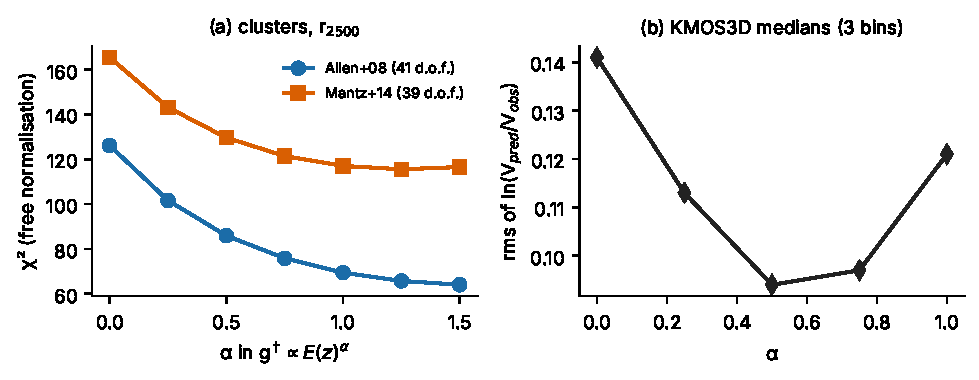
\includegraphics[width=\linewidth]{fig2_alpha.pdf}\end{minipage}\hfill\begin{minipage}[t]{0.40\textwidth}\centering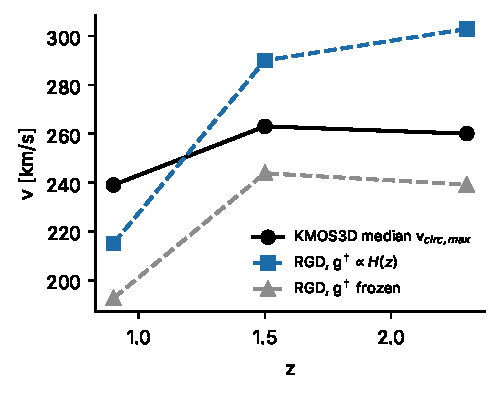
\includegraphics[width=\linewidth]{fig4_highz.pdf}\end{minipage}
\caption{Left: $\chi^2(\alpha)$ for the two cluster samples (a) and rms of $\ln(v_{\rm pred}/v_{\rm obs})$ for the three KMOS$^{\rm 3D}$ bins (b). Right: median circular velocities against redshift.}
\label{fig:alpha}
\end{figure}

For $\gdag\propto H(z)$ the zero-point shift relative to $z=0$ is $-3.75\Delta\log v=-0.18$, $-0.28$, $-0.38$ dex in $\log M$ at fixed velocity for the three bins, a monotonic trend, while the observed offsets relative to the local baryonic Tully--Fisher relation are $-0.44$ (at $z\simeq0.9$) and $-0.27$ (at $z\simeq2.3$), non-monotonic. The rms of $\ln(v_{\rm pred}/v_{\rm obs})$ is 0.141 for $\alpha=0$, 0.113 (0.25), 0.094 (0.50), 0.097 (0.75) and 0.121 for $\alpha=1$. The galaxies therefore favour $\alpha\simeq0.5$--0.75 and the clusters $\alpha\gtrsim1$. The two are reconciled only if the high-redshift galaxy systematics (gas masses from scaling relations with 0.2 dex error and no atomic gas, pressure-support corrections of 0.1--0.2 dex, selection that changes the stellar mass across bins) are of order 10\% or more, which they are; with three bins we cannot decide whether $\alpha$ depends on system scale. The dark matter fractions inferred in $z\simeq2$ galaxies are lower than at $z=0$ (\"Ubler et al.\ 2017; Genzel et al.\ 2017), whereas a larger $\gdag$ at the same baryonic acceleration produces a larger $K$; this is the same tension seen from another side and has not been tested quantitatively here.

%--------------------------------------------------------------------
\section{Connecting galaxies to clusters: the $\xi$ switch}
\label{sec:switch}
The radial term cannot be applied to galaxies: in SPARC an exploratory $s=(\Delta/\Delta_{\rm out})^p$, with $\Delta$ taken from the rotation curve itself, degrades the rms from 0.148 to 0.158, 0.235 and 0.468 dex for $p=0.25$, 0.5 and 1, and the global fit favours $p\simeq0.09$. A switch based on the local density does not separate the regimes, because inner cluster radii reach galactic densities; the discriminator must be a property of the system. The compactness $\xi$ is such a property: SPARC haloes have $\xi\simeq0.004$--0.094 (under two halo mass assumptions), the 43 groups $\xi=0.136$--0.29, X-COP $0.34$--0.54 and the Allen/Mantz clusters $0.40$--0.85. A step $\Theta(\xi-\xi_c)$ therefore needs $0.09\lesssim\xi_c\lesssim0.14$, a bracket set by the absence of systems in $0.09<\xi<0.136$. A saturating switch such as $1-e^{-\xi/0.052}$, the form inherited from $\alpha(\xi)$ in Paper~I, turns the term on partially at galactic $\xi$ and was found incompatible with the SPARC residuals in our test.

Because $\xi\propto(M_{500}H)^{1/3}$ the switch predicts a redshift-dependent threshold mass,
\begin{center}\small
\begin{tabular}{lccc}
\toprule
$M_{500}^{\rm thr}$ [$\Msun$] & $z=0$ & $z=1$ & $z=2$ \\
\midrule
$\xi_c=0.09$ & $4.2\times10^{12}$ & $2.4\times10^{12}$ & $1.4\times10^{12}$ \\
$\xi_c=0.14$ & $1.6\times10^{13}$ & $9\times10^{12}$ & $5.4\times10^{12}$ \\
\bottomrule
\end{tabular}
\end{center}
and, for the baryonic Tully--Fisher relation, a zero-point shift $\Delta\log v=0.25\log_{10}E(z)$ ($+0.061$ dex at $z=1$, $+0.118$ at $z=2$). The step itself is the simplest function that connects the regimes; its sharpness is unconstrained.

%--------------------------------------------------------------------
\section{Comparison with $\Lambda$CDM}
\label{sec:lcdm}
Table~\ref{tab:lcdm} compares the kernel with NFW haloes (Navarro et al.\ 1997) added to the same baryons, using either the concentration--mass relation of Duffy et al.\ (2008) or a free concentration.

\begin{table}[h]
\centering\footnotesize\setlength{\tabcolsep}{3.5pt}
\begin{tabular}{p{2.2cm}p{4.4cm}cccp{1.9cm}}
\toprule
Regime & Model & free par. & rms [dex] & AIC & note \\
\midrule
SPARC, 141 gal.\ & RGD kernel, $s=1$ & 0 & 0.142 & $-10670$ & \\
(2736 pts) & NFW + Duffy $c(M)$ & 141 & 0.087 & $-13066$ & \\
 & NFW, $c$ free & 282 & 0.059 & $-14877$ & \\
\midrule
SPARC, 175 gal.\ & RGD kernel & 0 & 0.148 & --- & 2803 pts \\
 & RAR, $a_0=1.2\times10^{-10}$ & 0 & 0.144 & --- & \\
 & Newton & 0 & 0.518 & --- & \\
\midrule
Groups (43) & NFW + Duffy, norm.\ to $M_{500}$ & 0 & 0.089 & --- & mean $-0.020$ \\
 & RGD, $p=0.5$, stars 9\% & 0 & 0.131 & --- & mean $-0.118$ \\
 & RGD, $p=0.8$, stars 9\% & 1 & 0.056 & --- & mean $-0.001$ \\
\midrule
X-COP, 39 pts & RGD $p=0.5$ / fitted & 0 / 1 & 0.021 / 0.016 & $-301$ / $-321$ & Table~\ref{tab:xcop} \\
 & NFW + Duffy & 13 & 0.039 & $-227$ & \\
\bottomrule
\end{tabular}
\caption{Kernel against $\Lambda$CDM haloes. Group numbers predict $M(<r_{2500})$ from $M_{500}$; the $\Lambda$CDM line has no free parameter. With realistic stellar masses ($\varphi=0.5$--0.7 of the Kravtsov relation) the groups prefer $p=0.45$--0.54; $\varphi$ is not measured. In the X-COP rows the observed baryon fraction is the scaling relation of Paper~I, not a measured profile.}
\label{tab:lcdm}
\end{table}

$\Lambda$CDM fits SPARC rotation curves better (0.087 or 0.059 against 0.142 dex), at the cost of one or two free parameters per galaxy; the kernel has none, and equals the RAR in quality (0.148 against 0.144). In groups $\Lambda$CDM with a $c(M)$ prior and no free parameter is better at $p=0.5$ with 9\% stars; the old-stellar-population value $p=0.8$ gives 0.056. In X-COP the radial term wins by AIC with a margin of 74 to 94 over NFW + Duffy, which has 12 more parameters, but this is within the calibration sample and with the Paper~I baryon fraction. A positive offset of $+0.15$ dex appears in SPARC galaxies with $V_{\max}<70\ {\rm km\,s^{-1}}$ (312 points, rms 0.25), which we find not to depend on $M_{\rm bar}$ and interpret as a selection effect of grouping by the observed maximum velocity. We therefore describe the kernel as competitive in clusters and parsimonious in galaxies, not as superior in fit.

%--------------------------------------------------------------------
\section{Tensions and tests that did not close}
\label{sec:tensions}
\paragraph{(1) Baryon fraction against mass at $r_{2500}$.} The kernel predicts $\fbar(r_{2500})$ rising with $M_{2500}$ by $+0.35$ per dex, against a measured mass slope of the observed fraction of $-0.04\pm0.09$ (Allen) and $-0.09\pm0.07$ (Mantz). In the Vikhlinin sample $\ln({\rm obs}/{\rm pred})$ has a trend of $-0.31$ per dex of $M_{2500}$ with $p=0.5$ (median obs/pred 0.84, rms$_{\ln}$ 0.225 over twelve clusters) and $-0.35$ with $p=0.46$ (0.76, 0.29). The effect worsens with realistic stellar masses and is independent of the form of $n(\xi)$.

\paragraph{(2) Absolute normalisation.} At $r_{500}$, where $p$ plays no role, obs/pred is 0.95 for Vikhlinin (Chandra) and 1.17 for X-COP (XMM-Newton), a $\sim20\%$ difference that is larger than the radial effect under test; at $r_{200}$ the X-COP value is 1.24. Known cross-calibration differences between the two instruments are of this order and were not modelled.

\paragraph{(3) A mass-dependent exponent.} The form $p(\xi)=p_0(\xi/0.4)^q$ with $q>0$ (bootstrap $q=0.37$ [0.31, 0.43], $p_0=0.46$ over Allen and Mantz) removes the trend of tension (1) ($-0.31\to-0.06$, Fig.~\ref{fig:trend}), but predicts a mass trend of $\fbar(r_{200})/\fbar(r_{500})$ of $+0.11$ against $-0.12$ observed and of the within-cluster $r_{2500}/r_{500}$ ratio of $-0.25$ against $-0.07$. It is not supported and is discarded as a hypothesis; the simplest reading remains constant $p\simeq0.5$.

\begin{figure}[h]
\centering
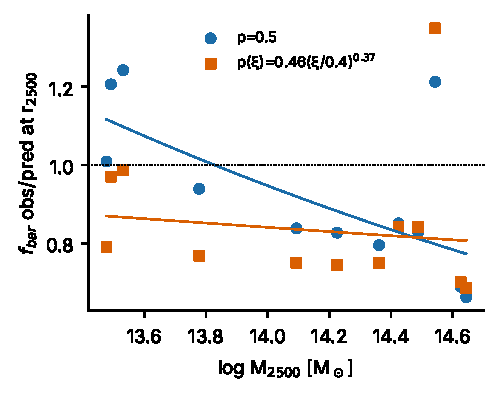
\includegraphics[width=0.48\textwidth]{fig3_mass_trend.pdf}
\caption{Vikhlinin et al.\ clusters: obs/pred baryon fraction at $r_{2500}$ against $\log M_{2500}$ for constant $p=0.5$ (trend $-0.31$ per dex) and for $p(\xi)\propto\xi^{0.37}$ (trend $-0.06$). Lines are log-linear fits.}
\label{fig:trend}
\end{figure}

\paragraph{(4) Hydrostatic equilibrium and lensing.} All cluster masses but CLASH are hydrostatic. Hydrostatic masses measure $g_{\rm obs}$ without bias if the gas is in equilibrium in the potential of Eq.~(\ref{eq:K}), but non-thermal pressure ($5.9\%$ at $r_{500}$ and $10.5\%$ at $r_{200}$ in X-COP) and departures from equilibrium were not modelled and the temperature and density profiles predicted by the kernel were not computed. A mass-dependent bias of the sign needed to close tension (1) would require hydrostatic masses to overestimate the true mass at high mass, opposite to the usual expectation from non-thermal pressure. Weighing-the-Giants calibration finds $M_L/M_X=0.96\,(+0.06/-0.09)\pm9\%$ (syst.) at $r_{2500}$, with a mass index $\beta=0.78\,(+0.17/-0.14)$ (assuming $M_L\propto M_X^\beta$), less than $2\sigma$ from 1 (Mantz et al.\ 2016); closing the trend would need $\beta\simeq0.87$. For the 12 clusters common to CLASH and Allen, $M_L/M_X(r_{2500})$ has median 1.21 (weighted mean 1.09, scatter 0.35 in $\ln$), obs/pred is 0.93 with lensing masses and 1.10 with X-ray masses (rms$_{\ln}$ 0.24 and 0.34). The lensing sample is small, high-mass and noisy, the gas was rescaled to the lensing aperture assuming $M_{\rm gas}\propto r^{1.2}$, and noise in $M_L$ enters both axes, so the mass trend itself is not informative there. Lensing calibration therefore reduces but does not decide the matter.

\paragraph{(5) High-redshift galaxies.} Sect.~\ref{sec:gz}.

%--------------------------------------------------------------------
\section{Extension to cosmological scales}
\label{sec:cosmo}
\subsection{The kernel applied to linear perturbations}
For a top-hat baryonic perturbation $\delta_b$ of physical radius $R$, $g_{\rm bar}=\tfrac12\Omega_b(a)H^2\delta_bR$ and
\begin{equation}
x=\frac{g_{\rm bar}}{\gdag}=\pi\,\Omega_b(a)\,\delta_b\,\frac{R}{c/H}.
\end{equation}
Over the history of the Universe and for $R=0.1$--100 Mpc comoving, $x=10^{-8}$--$4\times10^{-3}$, always deep in the low-acceleration regime. At $z=1100$ with $\delta_b=10^{-4}$, $K=7282$, 2303, 729 and 231 for $R=0.1,1,10,100$ Mpc, whereas mimicking cold dark matter needs $K=\Omega_m/\Omega_b=6.1$. A toy growth equation $\delta''+(2+d\ln H/d\ln a)\delta'=\tfrac32\Omega_b K(x(\delta))\delta$ from $z=1100$ gives $\delta(z=0)=123$, 127 and 134 for $\delta_i=10^{-5}$, $10^{-4}$, $10^{-3}$ at $R=10$ Mpc comoving (it scales as $1/R$: $1.2\times10^3$ at 1 Mpc, 13--15 at 100 Mpc), against 0.0076, 0.076 and 0.76 in $\Lambda$CDM. The result is nearly independent of the initial amplitude (the force scales as $\delta^{1/2}$), so the primordial amplitude $A_s$ would no longer control the spectrum and the fluctuations would not be linear and Gaussian. The toy neglects photon pressure and baryon--photon coupling before decoupling, which would delay growth, but the excess is $10^3$--$10^5$.

\subsection{Dilemma and damper}
If the kernel acts on cosmological perturbations it overshoots; if it acts only on bound systems, baryons alone grow by a factor 13 between $z=1100$ and today against 760 in $\Lambda$CDM ($\delta=0.013$ instead of 0.76 for $\delta_i=10^{-3}$) and no galaxy forms, and the CMB acoustic peaks cannot be produced without a potential well that does not couple to photons. A damper based on the baryon density contrast,
\begin{equation}
K_{\rm eff}=K_c\,(1-D)+K(x)\,D,\qquad D={\rm expit}\!\left[m\ln\frac{\rho_b/\rho_c}{\Delta_v}\right],\qquad K_c=\frac{\Omega_m}{\Omega_b}\simeq6.12,
\label{eq:damper}
\end{equation}
with $\Delta_v=30$ in $\rho_b/\rho_c$ (total $\Delta\simeq200$) and $m=4$ leaves bound systems unchanged and gives $\delta(z=0)=0.7604$ for $R=1$, 10 and 100 Mpc, identical to $\Lambda$CDM within $10^{-7}$ in the growth rate. This equality holds by construction, since $\rho_b/\rho_c\lesssim0.1$ in the linear regime and $D\to0$: it is consistent but not a test, and $K_c$ is a postulate. A hard cap $K\le K_c$ everywhere is excluded, since at $r_{500}$ the kernel already gives $K\simeq7.5>6.12$ ($\fbar=0.133$ against the cosmic 0.163); a cap would set $\fbar(r_{500})=0.163$ against the observed $\sim0.13$. That clusters sit below the cosmic baryon fraction without feedback is a qualitative consequence of $K>K_c$ in bound systems; we have not tested it against a specific measurement of the baryon depletion.

\subsection{CMB}
Reproducing the acoustic peaks requires a perturbation theory with baryon--photon coupling and a relativistic completion; kernel-type enhancements of the baryon force do not reproduce the third peak and the odd--even peak ratio, and the theories that do (e.g.\ Skordis \& Z\l{}o\'snik 2021) add a field that behaves as pressureless matter. We make no claim about the CMB or large-scale structure.

%--------------------------------------------------------------------
\section{Discussion}
\label{sec:disc}
\subsection{What the program claims}
\begin{enumerate}[leftmargin=2em,itemsep=0.1em]
\item In bound systems with symmetric equilibrium the kernel, with $\lambda$, $A$, $\gdag$ fixed on galaxies and groups, describes the baryon fraction across four orders of magnitude in mass with one radial parameter ($p\simeq0.45$--0.5) and one switch ($\xi_c\simeq0.09$--0.14).
\item The radial term $[\Delta/\Delta_{500}]^p$ replaces the two-parameter exponent modulation, reduces the X-COP rms from 0.037 to 0.016--0.021 dex and, unlike the former, extends to $r_{2500}$ and to $r_{200}$ on independent data.
\item $\gdag\propto H(z)$ is the preferred evolution in clusters and is not excluded in galaxies at $z\simeq1$--2 within current systematics.
\end{enumerate}
This is a phenomenological statement of restricted scope, defensible from the data used and not derived from a Lagrangian.

\subsection{What the program does not claim}
It does not claim that dark matter does not exist, nor that it replaces dark matter in cosmology: the CMB, linear growth and primordial perturbations are untouched, and the damper of Eq.~(\ref{eq:damper}) reproduces $\Lambda$CDM growth by postulate. It does not claim superiority in fit over $\Lambda$CDM haloes, which fit SPARC and, with the stellar assumption used, the groups better. The tensions of Sect.~\ref{sec:tensions} are open.

\subsection{Comparison with competing approaches}
Against MOND (Milgrom 1983) and the RAR (McGaugh et al.\ 2016) the transition scale evolves as $cH(z)/2\pi$ and the exponent depends on the compactness of the equilibrium; against $\Lambda$CDM the kernel is a baryon-only prescription with no per-system halo parameters in the tested regimes, but without cosmology. Observationally the two differ by the redshift evolution of the transition acceleration and by the dependence of the baryon fraction on $\xi$ and radius. Covariant relativistic MOND completions (e.g.\ AeST) address the CMB by adding a field; the kernel does not.

\subsection{Agenda for falsification}
\begin{enumerate}[leftmargin=2em,itemsep=0.1em]
\item \textbf{Radial parameter.} Resolved gas and lensing profiles (X-COP, eROSITA, XXL) should give $p=0.5\pm0.1$ independent of $\xi$ and mass; $|p-0.5|>0.15$ or a significant mass dependence falsifies the scale shift.
\item \textbf{Evolution of $\gdag$.} Clusters at $z>0.5$ with measured gas fractions (SPT, XMM) and larger samples of $z\simeq1$--2 rotation curves should converge on a common $\alpha$; independent samples preferring $\alpha<0.5$ at $2\sigma$ in clusters, or $\alpha>1$ in galaxies, falsify $\gdag\propto H(z)$.
\item \textbf{The switch.} Systems with $0.09<\xi<0.14$ must show a transition; galaxies with $\xi>0.14$ should show $s\neq1$, and systems with $\xi<0.09$ should show none. The threshold masses of Sect.~\ref{sec:switch} give the redshift dependence.
\item \textbf{Equilibrium in the kernel potential.} Predict $T(r)$ and $n_{\rm gas}(r)$ for the 12 X-COP and 12 Vikhlinin clusters in the potential of Eq.~(\ref{eq:K}) and compare with the measured profiles, including non-thermal pressure.
\item \textbf{Lensing at low mass.} Per-cluster lensing masses (CCCP, LoCuSS, WtG) below $M_{2500}\simeq2\times10^{14}\,\Msun$ to decide the mass trend of Sect.~\ref{sec:tensions}; measured $M_*(<r_{2500})$ in groups to fix $\varphi$.
\item \textbf{Systems not tested here.} El Gordo ($\xi\simeq0.73$) is an active merger and violates the equilibrium premise; ATLAS-3D/SLUGGS early-type galaxies and DESI rotation curves remain open from Paper~I.
\item \textbf{Covariant formulation.} Without an action the program has no predictions for gravitational waves, the CMB or strong fields.
\end{enumerate}

%--------------------------------------------------------------------
\section{Conclusions}
The kernel of Paper~I, extended with a one-parameter radial term, describes bound systems from galaxies to clusters better than before; it remains a phenomenological map, not a cosmological theory.

\paragraph{Established.}
\begin{enumerate}[leftmargin=2em,itemsep=0.1em]
\item The radial term is necessary: without it the kernel mispredicts the baryon fraction at $r_{2500}$ by a factor 3--4 and at $r_{200}$ by a factor 2.4.
\item $s=[\Delta/\Delta_{500}]^p$ with $p\simeq0.45$--0.5 describes it with one parameter: X-COP rms 0.126 $\to$ 0.016--0.021 dex (v4 law: 0.037), $\fbar(r_{2500})/\fbar(r_{500})$ predicted 1.00 against 0.90 observed, $\fbar(r_{200})/\fbar(r_{500})$ 0.97 against 1.03.
\item The v4 law $w^{-\alpha(\xi)}$ is adequate for $w\gtrsim0.7$ in X-COP but fails inside $r_{500}$ ($n>1$) and does not meet the v4 criterion of 0.10 dex at $r_{2500}$.
\item $\gdag\propto H(z)$ is preferred by Allen and Mantz gas fractions; a frozen $\gdag$ costs $\Delta\chi^2=57$ and 48.
\item A step in $\xi$ at $\xi_c=0.09$--0.14 connects galaxies, groups and clusters, with redshift-dependent threshold masses ($4\times10^{12}$ to $1.4\times10^{12}\,\Msun$ from $z=0$ to 2 for $\xi_c=0.09$).
\end{enumerate}

\paragraph{Not established.}
\begin{enumerate}[leftmargin=2em,itemsep=0.1em]
\item The baryon fraction at $r_{2500}$ rises with mass more than observed ($-0.31$ per dex in obs/pred); lensing calibration shifts it by $\sim1\sigma$.
\item The absolute normalisation differs by $\sim20\%$ between the Chandra and XMM samples (0.95 against 1.17 at $r_{500}$).
\item A mass-dependent $p(\xi)\propto\xi^{0.37}$ closes the former but predicts the wrong sign of the $r_{500}\to r_{200}$ trend, and is discarded.
\item Median KMOS$^{\rm 3D}$ galaxies prefer $\gdag\propto E^{0.5\text{--}0.75}$ against $\alpha\gtrsim1$ in clusters, within the $\sim10\%$ systematics of the former.
\item Applied to linear perturbations the kernel boosts gravity $10^2$--$10^3$ times; the damper recovers $\Lambda$CDM growth only through the postulated plateau $K_c=\Omega_m/\Omega_b$; no CMB statement is made.
\end{enumerate}

\paragraph{Position relative to $\Lambda$CDM.} In clusters the kernel is competitive (X-COP AIC $-301$ to $-321$ against $-227$, in-sample); in galaxies it is parsimonious (zero parameters) but fits worse than haloes (0.142 against 0.087 or 0.059 dex); in groups $\Lambda$CDM is better for $p=0.5$ with the stellar assumption used; in cosmology the kernel makes no competitive claim. The defensible claim is an empirical map of bound systems that any covariant theory must reproduce in the weak-field stationary limit.

%--------------------------------------------------------------------
\section*{Data and code availability}
All scripts, the transcribed tables and the figure generator are in the public repository \url{https://github.com/Maia-KarlosMarden/rgd-kernel} (folder \texttt{v5}). SPARC, X-COP, CLASH, Allen, Mantz, Vikhlinin, Lovisari, Sun and KMOS$^{\rm 3D}$ data are public from the original publications; the transcribed tables should be checked against the originals before reuse.

\section*{Acknowledgements}
The author thanks the teams behind the public datasets used here: SPARC (F.~Lelli, S.~McGaugh, J.~Schombert), X-COP (S.~Ettori, V.~Ghirardini, D.~Eckert), CLASH (K.~Umetsu et al.), KMOS$^{\rm 3D}$ (H.~\"Ubler et al.), and the authors of the cluster compilations of Allen, Mantz, Vikhlinin, Lovisari, Sun, Kravtsov and Gonzalez. No grant funding supported this work. \emph{AI assistance:} the analysis scripts, the numerical cross-checks and the drafting of this manuscript were carried out with the assistance of Claude (Anthropic); the scientific choices and the responsibility for the content are the author's.

%--------------------------------------------------------------------
\appendix
\section{Reproducibility notes}
\label{app:repro}
\begin{itemize}[leftmargin=2em,itemsep=0.1em]
\item Scripts are run from inside the \texttt{v5} folder (several use \texttt{exec(open(\dots))}); \texttt{v4\_vs\_v5.py} reproduces Table~\ref{tab:xcop}, \texttt{v4\_indep.py} the independent radial tests, \texttt{alpha\_scan.py} Table~\ref{tab:alpha}, \texttt{highz\_tf.py} Table~\ref{tab:highz}, \texttt{lcdm\_compare.py} Table~\ref{tab:lcdm}, \texttt{cmb\_regime.py} and \texttt{damper\_test.py} Sect.~\ref{sec:cosmo}.
\item SPARC Table 2 is not redistributed; set the environment variable \texttt{SPARC\_TABLE2}.
\item Mantz fractions are shell values and Allen and Vikhlinin cumulative; Mantz $M_{2500}$ was validated against the critical-density definition, Vikhlinin $M_{500}$ likewise. Cosmology: flat, $H_0=70$, $\Omega_m=0.3$ throughout except where stated (Vikhlinin: $h=0.71$; CLASH: $\Omega_m=0.27$; the differences were not propagated).
\item The X-COP rows labelled ``scaling'' follow Paper~I's $f_{\rm bar}=1.09\fgas(M_{500})$ with $\fgas=0.0708(M_{500}/10^{13}\Msun)^{0.135}$; the measured-profile test is the Ettori et al.\ Table~2 analysis.
\end{itemize}

%--------------------------------------------------------------------
\begin{thebibliography}{99}
\setlength{\itemsep}{0.1em}
\bibitem[Allen et al.(2008)]{allen08} Allen, S.~W., Rapetti, D.~A., Schmidt, R.~W., et al.\ 2008, MNRAS, 383, 879
\bibitem[Duffy et al.(2008)]{duffy08} Duffy, A.~R., Schaye, J., Kay, S.~T., \& Dalla Vecchia, C.\ 2008, MNRAS, 390, L64
\bibitem[Eckert et al.(2019)]{eckert19} Eckert, D., Ghirardini, V., Ettori, S., et al.\ 2019, A\&A, 621, A40
\bibitem[Ettori et al.(2019)]{ettori19} Ettori, S., Ghirardini, V., Eckert, D., et al.\ 2019, A\&A, 621, A39 (arXiv:1805.00034)
\bibitem[Genzel et al.(2017)]{genzel17} Genzel, R., F\"orster Schreiber, N.~M., \"Ubler, H., et al.\ 2017, Nature, 543, 397
\bibitem[Ghirardini et al.(2019)]{ghirardini19} Ghirardini, V., Eckert, D., Ettori, S., et al.\ 2019, A\&A, 621, A41
\bibitem[Gonzalez et al.(2013)]{gonzalez13} Gonzalez, A.~H., Sivanandam, S., Zabludoff, A.~I., \& Zaritsky, D.\ 2013, ApJ, 778, 14 (arXiv:1309.3565)
\bibitem[Kravtsov et al.(2018)]{kravtsov18} Kravtsov, A.~V., Vikhlinin, A.~A., \& Meshcheryakov, A.~V.\ 2018, Astronomy Letters, 44, 8 (arXiv:1401.7329)
\bibitem[Lelli et al.(2016)]{lelli16} Lelli, F., McGaugh, S.~S., \& Schombert, J.~M.\ 2016, AJ, 152, 157
\bibitem[Lovisari et al.(2015)]{lovisari15} Lovisari, L., Reiprich, T.~H., \& Schellenberger, G.\ 2015, A\&A, 573, A118
\bibitem[Maia(2026)]{maia26} Maia, K.\ 2026, \emph{A Cosmological-Background Effective Gravitational Kernel: Unifying disk galaxies, galaxy groups, galaxy clusters, and gravitational lensing under a single effective law}, v4 (April 28, 2026)
\bibitem[Mantz et al.(2014)]{mantz14} Mantz, A.~B., Allen, S.~W., Morris, R.~G., et al.\ 2014, MNRAS, 440, 2077
\bibitem[Mantz et al.(2016)]{mantz16} Mantz, A.~B., Allen, S.~W., Morris, R.~G., et al.\ 2016, \emph{Cosmology and astrophysics from relaxed galaxy clusters --- IV. Robustly calibrating hydrostatic masses with weak lensing}, MNRAS (arXiv:1509.02162)
\bibitem[McGaugh et al.(2016)]{mcgaugh16} McGaugh, S.~S., Lelli, F., \& Schombert, J.~M.\ 2016, Phys.\ Rev.\ Lett., 117, 201101
\bibitem[Milgrom(1983)]{milgrom83} Milgrom, M.\ 1983, ApJ, 270, 365
\bibitem[Navarro et al.(1997)]{nfw97} Navarro, J.~F., Frenk, C.~S., \& White, S.~D.~M.\ 1997, ApJ, 490, 493
\bibitem[Skordis \& Z\l{}o\'snik(2021)]{skordis21} Skordis, C., \& Z\l{}o\'snik, T.\ 2021, Phys.\ Rev.\ Lett., 127, 161302
\bibitem[Sun et al.(2009)]{sun09} Sun, M., Voit, G.~M., Donahue, M., et al.\ 2009, ApJ, 693, 1142
\bibitem[\"Ubler et al.(2017)]{ubler17} \"Ubler, H., F\"orster Schreiber, N.~M., Genzel, R., et al.\ 2017, ApJ, 842, 121 (arXiv:1703.04321)
\bibitem[Umetsu et al.(2016)]{umetsu16} Umetsu, K., Zitrin, A., Gruen, D., et al.\ 2016, ApJ, 821, 116 (arXiv:1507.04385)
\bibitem[Vikhlinin et al.(2006)]{vikhlinin06} Vikhlinin, A., Kravtsov, A., Forman, W., et al.\ 2006, ApJ, 640, 691
\end{thebibliography}

\end{document}
